\section*{28. Дивергенция магнитного поля. Вектор-потенциал. Кулоновская
калибровка.}
 
\subsection*{Дивергенция магнитного поля}

\noindent
\begin{minipage}[c]{0.2\textwidth} % Левая часть: изображение
    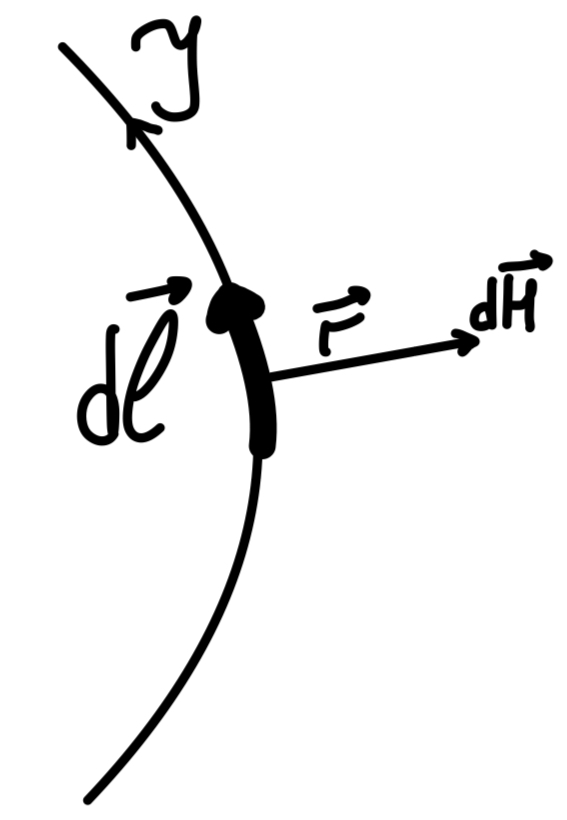
\includegraphics[width=\textwidth]{im/62.png}{} % Ваше изображение
\end{minipage}%
\hfill
\begin{minipage}[c]{0.68\textwidth} % Правая часть: текст
    
    \( d\vec{H}=\frac{I}{c}\left[ d\vec{l}\times \frac{\vec{r}}{r^3}  \right] \text{ Надо доказать, что: }\mathrm{div} \vec{H}=0 \)
    
    Принцип суперпозиции: $\vec{H}=\int d\vec{H}$
    
    Достаточно доказать, что $\mathrm{div} d\vec{H}$, так как $\mathrm{div}-$линеный оператор. 
\end{minipage}

\[
d\vec{H}=\frac{I}{c}\left[d\vec{l}\times \left( -\grad\left( \frac{1}{r}  \right) \right)\right] 
\]

Напомним: 

\[
\grad \left( \frac{1}{r}\right)=-\frac{1}{r^2}\grad(r)=\frac{1}{r^2}\frac{\vec{r}}{r} 
\]

\[
\mathrm{div}d\vec{H}=\frac{I}{c}\grad \left[ d\vec{l}\times \left( -\grad \left( \frac{1}{r}  \right) \right) \right]=\frac{I}{c}\left( d\vec{l} \underbrace{\left[ \grad \times \grad\left( \frac{1}{r}  \right) \right]}_{=0} \right) =0  
\]

\noindent
\begin{minipage}[c]{0.35\textwidth} % Левая часть: изображение
    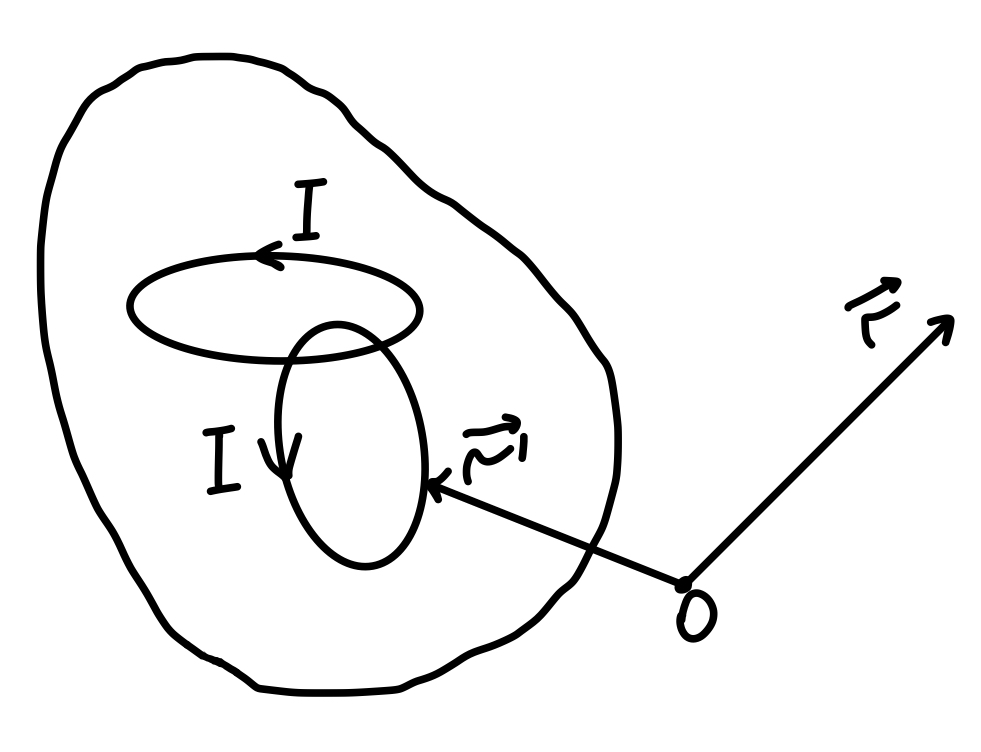
\includegraphics[width=\textwidth]{im/63.png}{} % Ваше изображение
\end{minipage}%
\hfill
\begin{minipage}[c]{0.7\textwidth} % Правая часть: текст
   
    \[
    \begin{array}{l|l}
        \vec{H}=\sum_{i} \frac{I_i}{c}\int \left[ d\vec{r'}\times \frac{\vec{r}-\vec{r'}}{|\vec{r}-\vec{r'}|^3}  \right] & \Rightarrow \\
        d\vec{l}\equiv d\vec{r'} & \\
        Id\vec{l}=\vec{j}dV' & \\
    \end{array}
    \]

\end{minipage}

\[
\begin{array}{|l}
    \Rightarrow \text{ т.о }\vec{H}=\underset{V}{\iiint}\frac{1}{c} \frac{[\vec{j}\times (\vec{r}-\vec{r'})]}{|\vec{r}-\vec{r'}|^3}dV' \\ 
    \vec{H}= \frac{1}{c} \underset{V}{\iiint} \left[ \vec{j}\times \left( -\frac{1}{|\vec{r}-\vec{r'}|} \right) \right]dV'
\end{array}
\]

Напомним: 

\[
\grad:=\frac{\partial}{\partial \vec{r}}; \grad ' := \frac{\partial}{\partial \vec{r'}}
\]

\[
\mathrm{div}\vec{H}=\frac{1}{c}\underset{V}{\iiint}\left( \grad \left[ \vec{j} \times \grad \left( -\frac{q}{|\vec{r}-\vec{r'}|}  \right) \right] \right)dV'= \frac{1}{c}\underset{V}{\iiint}\left( \vec{j}\underbrace{\left[ \grad \times \grad \frac{1}{|\vec{r}-\vec{r'}|}  \right]}_{=0} \right)dV'
\]

\subsection*{Вектор-потенциал}

$\mathrm{div}\vec{H}=0\Rightarrow \vec{H} $ можно подставить в виде $\mathrm{rot} $ некоторого вектора.

\[
\vec{H}\overset{df}{=}\mathrm{rot}\vec{A} 
\]

Определить вектор поля одним только $\mathrm{rot} $ нельзя. 

\[
\begin{aligned}
    \begin{array}{l|l}
        \begin{cases}
            \mathrm{div}\vec{A_1}=\mathrm{div}\vec{A_2} \qquad \vec{A}=\vec{A_1}-\vec{A_2} \\
            \mathrm{rot}\vec{A_1}=\mathrm{rot}\vec{A_2}    
        \end{cases}   
    \end{array}
    \Rightarrow
    \begin{cases}
        \mathrm{div}\vec{A}=0 \\
        \mathrm{rot}\vec{A}=0 \Rightarrow \vec{A}=-\grad\varphi 
    \end{cases}
\end{aligned}
\]

\[
\begin{cases}
    \vec{A}=\grad\varphi \\
    \Delta\varphi=0
\end{cases}
\]

Можно взять $\vec{A}=\frac{1}{c}\underset{V}{\iiint} \frac{\vec{j}(\vec{r'})}{|\vec{r}-\vec{r'}|}dV'$( где $V$ предыдущий объём)

Покажем, что $\mathrm{rot}\vec{A}=\vec{H} \text{ и } \mathrm{div}\vec{A}=0: $

\[
\mathrm{rot}\vec{A}=\frac{1}{c}\underset{V}{\iiint} \left[ \grad \times \frac{\vec{j}(\vec{r'})}{|\vec{r}-\vec{r'}|}  \right]dV'=\frac{1}{c}\iiint \left[ \vec{j}\times \left( -\frac{1}{|\vec{r}-\vec{r'}|}  \right) \right] dV'=\vec{H} \quad \blacksquare
\]

\[
\mathrm{div}\vec{A}=\frac{1}{c}\underset{V}{\iiint}\grad \vec{j}\frac{1}{|\vec{r}-\vec{r'}|}dV'=\frac{1}{c}\underset{V}{\iiint} \vec{j}\grad \frac{1}{|\vec{r}-\vec{r'}|}dV'\fbox{=}
\]

Уточнение:

\[
\grad \frac{1}{|\vec{r}-\vec{r'}|}=-\grad ' \frac{1}{|\vec{r}-\vec{r'}|}  
\]
 
\[
\fbox{=}-\frac{1}{c}\underset{V}{\iiint}\vec{j}(\vec{r'})\grad ' \overset{\downarrow}{\frac{1}{{|\vec{r}-\vec{r'}|}}}dV'=-\frac{1}{c}\underset{V}{\iiint}\overset{\downarrow}{\vec{j}}(\vec{r'})\grad ' \overset{\downarrow}{\frac{1}{|\vec{r}-\vec{r'}|} }dV'+
\]

\[
    +\frac{1}{c}\underset{V}{\iiint}\overset{\downarrow}{\vec{j}}(\vec{r'})\grad ' \frac{1}{{|\vec{r}-\vec{r'}|}}dV'\fbox{=}
\]

\newpage

\[
\fbox{=}-\frac{1}{c}\underset{V}{\iiint} \mathrm{div} \left( \frac{\vec{j}(\vec{r'})}{|\vec{r}-\vec{r'}|} \right) dV'+\frac{1}{c}\underset{V}{\iiint}\frac{1}{|\vec{r}-\vec{r'}|}\mathrm{div}(\cancelto{0}{\vec{j}(\vec{r'})})dV'\fbox{=}
\]

\[
\fbox{=}\underbrace{-\frac{1}{c}\underset{\delta V}{\oiint} \frac{\cancelto{0}{\vec{j}(\vec{r'})}}{|\vec{r}-\vec{r'}|}dS'}_{\text{на границе нет токов}}+\underbrace{0}_{\text{по З.С.З}}=0 \quad \blacksquare
\]

Закон сохранения заряда:

\[
\frac{\partial \rho}{\partial t} +\mathrm{div}\vec{j}=0 \text{, стационарный случай } \left( \frac{\partial \rho}{\partial t}  \right)=0 \Rightarrow \mathrm{div}\vec{j}=0  
\]

\textit{Ротор магнитного тока:}

\[
(\overset{a}{\grad}\times[\overset{b}{\grad}\times \overset{c}{\vec{A}}])\overset{bac-cab}{=}\grad\cdot[\grad\cdot\vec{A}]-(\grad\cdot\grad)\cdot\vec{A}
\]

Вспомним $\mathrm{rot}(\mathrm{rot}\vec{A})=\mathrm{grad}(\mathrm{div}\vec{A})-\Delta \vec{A}$

\[
\begin{aligned}
    \begin{array}{l|l}
        \vec{H}=\mathrm{rot}\vec{A}, \\ 
        \text{где }\vec{A}=\frac{1}{c}\underset{V}{\iiint}\frac{\vec{j}(\vec{r'})}{|\vec{r}-\vec{r'}|}  
    \end{array}
    \Rightarrow \mathrm{rot}\vec{H}=  \mathrm{rot}(\mathrm{rot}\vec{A} )= \mathrm{grad}(\cancelto{0}{\mathrm{div}\vec{A} })-\Delta\vec{A} \fbox{=} \\
\end{aligned}
\]

\[
\fbox{=}\frac{1}{c}\underset{V}{\iiint}\vec{j}(\vec{r'})\Delta \frac{1}{|\vec{r}-\vec{r'}|}dV'=\frac{1}{c}\underset{V}{\iiint}\vec{j}(\vec{r'})4\pi\delta(\vec{r}-\vec{r'})dV' = 
\]

\[
=\frac{4\pi}{c}\underset{V}{\iiint}\vec{j}(\vec{r'})\delta (\vec{r}-\vec{r'})dV'=\frac{4\pi}{c}\vec{j}(\vec{r})  
\]

\[
\text{Итог: } \boxed{\mathrm{rot}\vec{H}=\frac{4\pi}{c}\vec{j}  }
\]

\subsection*{Кулоновская калибровка}

\textit{Кулоновская калибровка} — выбор векторного потенциала магнитного поля $\vec{A}$ с дополнительным условием

\[
\mathrm{div}\vec{A}=0 
\]

Эта калибровка применяется для рассмотрения нерелятивистских магнитостатических задач.